\documentclass{beamer}


\usepackage{amsmath,amssymb}

\usepackage{tikz}
\usepackage{booktabs}
\usepackage{graphicx}

\usetikzlibrary{calc}
\usetikzlibrary{shapes}
\usetikzlibrary{arrows}
\usetikzlibrary{backgrounds}

\setbeamertemplate{navigation symbols}{}

\begin{document}

\frame{
\begin{center}
\href{https://plus.google.com/+VincentKnight/posts}{+Vincent.Knight}\\
\href{https://twitter.com/drvinceknight}{@drvinceknight}\\
\href{http://drvinceknight.github.io/Talks/}{vincent-knight.com/Talks}\\
\end{center}
}

\frame{
    \Huge
    \[
        \begin{pmatrix}
        (2,2)&(5,0)\\
        (0,5)&(4,4)
        \end{pmatrix}
    \]
}


\frame{

    \begin{center}

    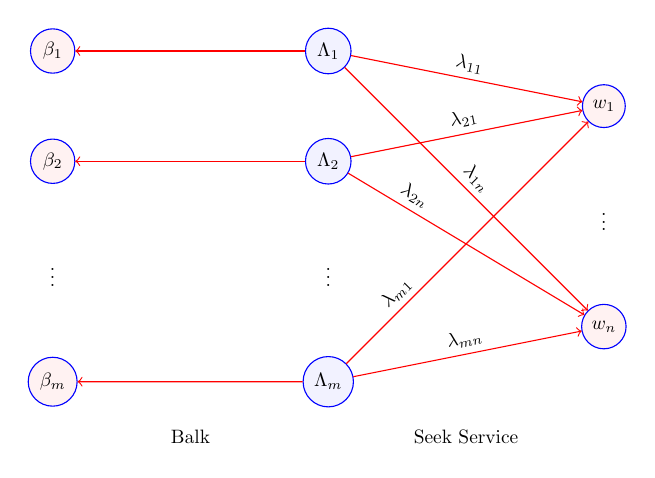
\begin{tikzpicture}[scale=0.7, every node/.style={scale=0.7}]
        \node (S1) at (0,0) [circle, draw=blue, fill=blue!5] {$\Lambda_1$};
    \node (S2) at (0,-2) [circle, draw=blue, fill=blue!5] {$\Lambda_2$};
    \node (S3) at (0,-4)  {$\vdots$};
    \node (S4) at (0,-6) [circle, draw=blue, fill=blue!5] {$\Lambda_m$};

    \node (B1) at (-5,0) [circle, draw=blue, fill=red!5] {$\beta_1$};
    \node (B2) at (-5,-2) [circle, draw=blue, fill=red!5] {$\beta_2$};
    \node (B3) at (-5,-4)  {$\vdots$};
    \node (B4) at (-5,-6) [circle, draw=blue, fill=red!5] {$\beta_m$};

    \node (F1) at (5,-1) [circle, draw=blue, fill=red!5] {$w_1$};
    \node (F3) at (5,-3)  {$\vdots$};
    \node (F2) at (5,-5) [circle, draw=blue, fill=red!5] {$w_n$};

    \draw [->, red] (S1) -- (B1);
    \draw [->, red] (S2) -- (B2);
    \draw [->, red] (S4) -- (B4);

    \draw [->, red] (S1) -- (F1) node [midway, above, sloped, black] (TextNode) {$\lambda_{11}$};
    \draw [->, red] (S1) -- (F2) node [midway, above, sloped, black] (TextNode) {$\lambda_{1n}$};
    \draw [->, red] (S2) -- (F1) node [midway, above, sloped, black] (TextNode) {$\lambda_{21}$};
    \draw [->, red] (S2) -- (F2) node [near start, above, sloped, black] (TextNode) {$\lambda_{2n}$};
    \draw [->, red] (S4) -- (F1) node [near start, above, sloped, black] (TextNode) {$\lambda_{m1}$};
    \draw [->, red] (S4) -- (F2) node [midway, above, sloped, black] (TextNode) {$\lambda_{mn}$};

    \node at (-2.5,-7) {Balk};
    \node at (2.5,-7) {Seek Service};
    \end{tikzpicture}
    \end{center}
}

\frame{
    \begin{center}
    \begin{tabular}{cl}
    \toprule
        Parameter                              & Interpretation\\
        \midrule
        $m\in\mathbb{Z}$                       & Number of sources\\
        $n\in\mathbb{Z}$                       & Number of service centers\\
        $\beta\in\mathbb{R}_{\geq 0}^{m}$      & Worth of service\\
        $\Lambda\in\mathbb{R}_{\geq 0}^{m}$    & Demand rate\\
        $w_j$ for $j\in[n]$                    & A convex utility function\\
        $d_{ij}$ for $i\in[m],\;j\in[n]$       & Distance from source $i$ to service center $j$\\
        $\lambda_{ij}$ for $i\in[m],\;j\in[n]$ & Traffic from source $i$ to service center $j$\\
        \toprule
        \end{tabular}
    \end{center}
}

\frame{
    \begin{center}

    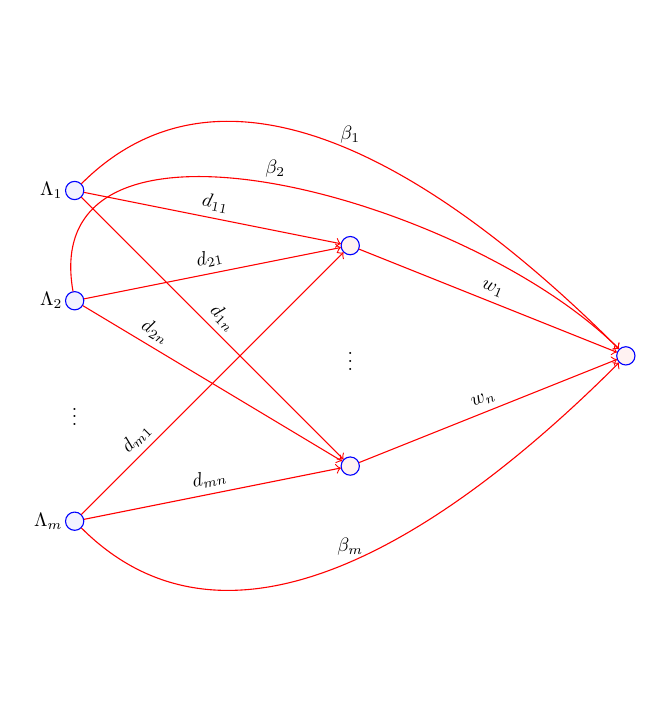
\begin{tikzpicture}[scale=0.7, every node/.style={scale=0.7}]
        \node (S1) at (0,0) [circle, draw=blue, fill=blue!5] {} node[left=.1cm] {$\Lambda_1$};
    \node (S2) at (0,-2) [circle, draw=blue, fill=blue!5] {} node at (S2)[left=.1cm] {$\Lambda_2$};
    \node (S3) at (0,-4)  {$\vdots$};
    \node (S4) at (0,-6) [circle, draw=blue, fill=blue!5] {} node at (S4) [left=.1cm] {$\Lambda_m$};

    \node (E) at (10,-3) [circle, draw=blue, fill=red!5] {};

    \node (F1) at (5,-1) [circle, draw=blue, fill=red!5] {};
    \node (F3) at (5,-3)  {$\vdots$};
    \node (F2) at (5,-5) [circle, draw=blue, fill=red!5] {};

    \draw [->, red] (F1) -- (E) node [midway, above, sloped, black] (TextNode) {$w_{1}$};
    \draw [->, red] (F2) -- (E) node [midway, above, sloped, black] (TextNode) {$w_{n}$};


    \draw [->, red] (S1) -- (F1) node [midway, above, sloped, black] (TextNode) {$d_{11}$};
    \draw [->, red] (S1) -- (F2) node [midway, above, sloped, black] (TextNode) {$d_{1n}$};
    \draw [->, red] (S2) -- (F1) node [midway, above, sloped, black] (TextNode) {$d_{21}$};
    \draw [->, red] (S2) -- (F2) node [near start, above, sloped, black] (TextNode) {$d_{2n}$};
    \draw [->, red] (S4) -- (F1) node [near start, above, sloped, black] (TextNode) {$d_{m1}$};
    \draw [->, red] (S4) -- (F2) node [midway, above, sloped, black] (TextNode) {$d_{mn}$};

    \draw [->, red] (S1) edge[out=45, in=135] node [above, black] {$\beta_1$} (E);
    \draw [->, red] (S4) edge[out=-45, in=-135] node [above, black] {$\beta_m$} (E);
    \draw [->, red] (S2) edge[out=100, in=135] node [above, black] {$\beta_2$} (E);

    \end{tikzpicture}
    \end{center}
}

\frame{

    \begin{center}
    \begin{tikzpicture}

    \draw [->] (0,0) -- (10,0);
    \draw [->] (0,0) -- (0,8);
    \node at (10,0) [below] {$\Lambda$};
    \node at (0,8) [left] {PoA};

    %\node (social) at (3,0) [below] {$x^*$};
    %\node (selfish) at (7,0) [below] {$\tilde x$};

    \draw [dashed] (3,0) -- (3,8);
    \draw [dashed] (7,0) -- (7,8);

    \draw [thick] (0,3) -- (3,3);
    \draw (3,3) edge[thick,out=0,in=-100] (7,6);
    \draw (7,6) edge[thick,out=-80,in=170] (10,4);

    \node at (1.5,4) [text width=2cm]{Low level of demand};
    \node at (5,6) {Inefficient system};
    \node at (8.5,2) [text width=2cm]{High level of demand};

    \end{tikzpicture}

    \end{center}
}
\end{document}
